% master file siminos/froehlich/slice/chart.tex
% $Author$ $Date$

% \section{Charting the \reducedsp}
%       \label{sec:chart}


So far, the good news is that for a generic {\template} $\slicep$ (\ie,
any $\slicep$ whose group orbit has the full $N$-dimensions of the
symmetry group \Group), the slice hyperplane \refeq{PCsectQ} cuts across
the group orbit of {\em every} point in the full \statesp\ \pS. But is
this a useful symmetry reduction of the full \statesp? A distant pattern
that is a bad match to a given {\template} will have any number of
locally `minimal' distances, each yet another bad match. It makes no
sense physically to use one slice (a set of all group orbit points that
are closest to one given {\template}) globally.

Work on \KS\ suggests how to proceed: it was shown in
\refrefs{lanCvit07,SCD07} that for turbulent/chaotic systems a set of
Poincar\'e sections is needed to capture the dynamics. The choice should
be physical, dictated by the dominant patterns seen in the solutions of
nonlinear PDEs. We propose to construct a global chart of the
$\pS/\Group$ symmetry \reducedsp\ by deploying both linear slices and
linear Poincar\'e sections across neighborhoods of the most important
(relative) equilibria and/or (relative) periodic orbits (taking care that
the {\template s} chosen have no symmetry). Each slice $\pSRed{}^{(j)}$,
tangential to one of a finite number of {\template s}  $\slicep{}^{(j)}$,
captures a neighborhood of an important, qualitatively distinct class of
solutions (2-rolls states, 3-rolls states, \etc); together they `Voronoi'
tessellate  the curved manifold in which the reduced strange attractor is
embedded by a finite set of hyperplane tiles\rf{RoSa00}. This is the
symmetry-reduced generalization of the idea of {\statesp\ tessellation}
by a set of periodic-orbits, so dear to a professional cyclist,
\reffig{fig:Tesselate}.

So how do we propose to implement this tessellation?

The physical task is to, for a given dynamical flow, pick a set of
{\template s} with slices approximately tangent to the strange attractor.
A `slice' is a purely group-theoretic, linear construct, with no
reference to dynamics; a given {\template} $\slicep{}^{(1)}$ defines the
associated slice $\pSRed$, a ($d\!-\!1$)\dmn\ tangent hyperplane (for
simplicity, in this section we specialize to the $\SOn{2}$ case). Within
it, there is a ($d\!-\!2$)\dmn\ {\sset} \refeq{sliceSingl}. If we pick
another {\template} point $\slicep{}^{(2)}$, it comes along with its own
slice and {\sset}. Any neighboring pair of $(d\!-\!1)$\dmn\ slices
intersects in a `ridge' (`boundary,' `edge'), a $(d\!-\!2)$\dmn\
hyperplane, easy to compute, which goes through the `origin,' or, more
precisely, the fixed-point subspace  $\pS_\Group$. So all intersections
of slices, ridges and {\sset s} contain the fixed-point subspace
$\pS_\Group$. Global atlas so constructed should be sufficiently
fine-grained that we never hit any slice singularities. Each
neighborhood, bounded by ridges to neighboring slices, should be
sufficiently small so that {\sset} is nowhere within the part of the
slice explored by the strange attractor. The {\sset}s should be
eliminated by requiring that they lie either on the far sides of the
slice-slice intersections, or elsewhere where the strange attractor does
not tread.




% In FrCv11.tex replaced by f_1_08_1.png
%{Hyp} %{fig6} and {tr:fig6} in ChaosBook
% \HREF{http://chaosbook.org/overheads/trace/Tesselate.jpg}
%%%%%%%%%%%%%%%%%%%%%%%%%%%%%%%%%%%%%%%%%%%%%%%%%%
 \begin{figure}
 \begin{center}
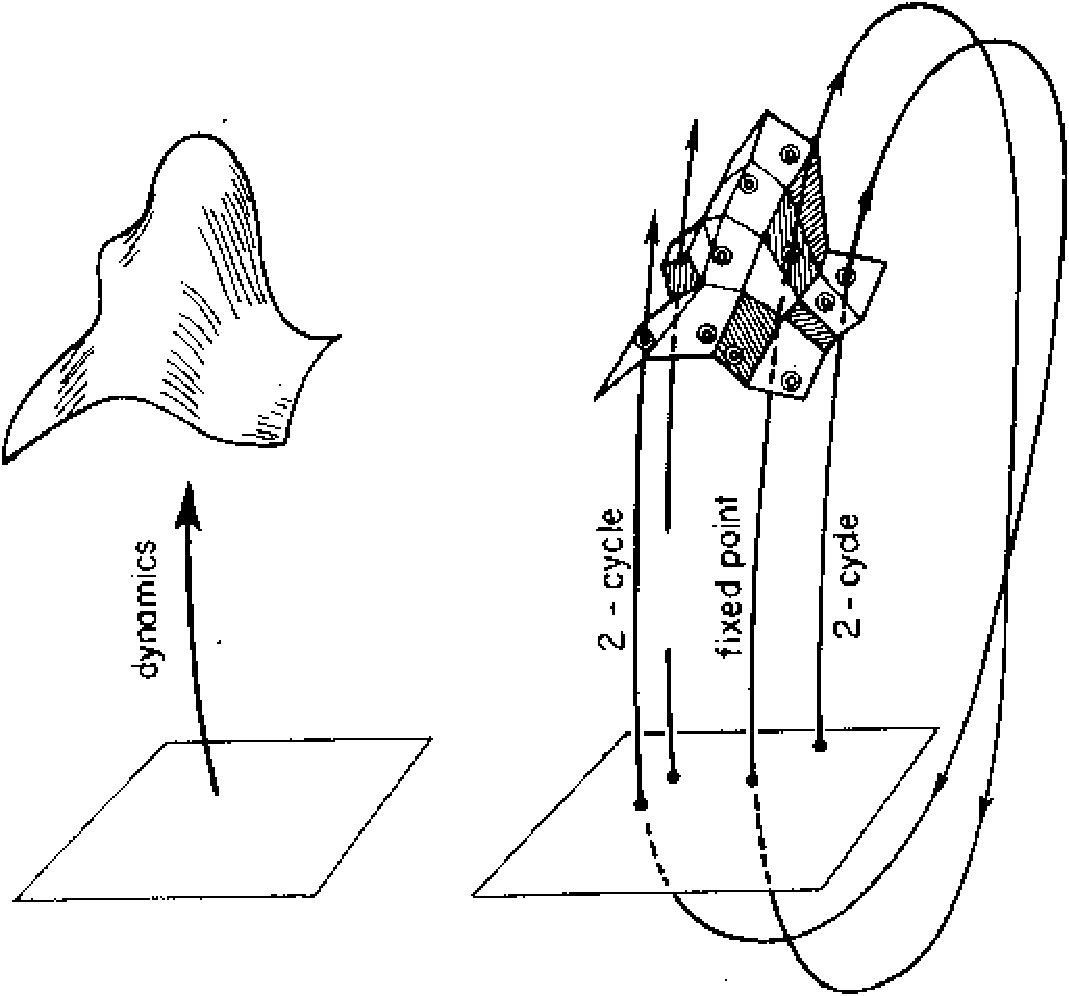
\includegraphics[width=0.35\textwidth]{f_1_08_1}
 \end{center}
 \caption{\label{fig:Tesselate}
Smooth dynamics  (left frame) tesselated by the skeleton of periodic
points, together with their linearized neighborhoods, (right frame).
Indicated are segments of two 1-cycles and a 2-cycle that alternates
between the neighborhoods of the two 1-cycles, shadowing first one, and
then the other
(from \wwwcb{}).
  }\end{figure}
%%%%%%%%%%%%%%%%%%%%%%%%%%%%%%%%%%%%%%%%%%%%%%%%%%
%



Follow an ant as it crawls along the symmetry-reduced trajectory
$\sspRed{}^{(1)}(\tau)$, within the slice $\pSRed{}^{(1)}$. The moment
$\braket{\sspRed{}^{(1)}(\tau)}{\sliceTan{}{}^{(2)}}$ changes sign, the
ant has crossed the ridge, we symmetry-reduce with respect to the second
slice, and the ant continues its merry stroll within $\pSRed{}^{(2)}$.
Or, if you prefer to track the  given full \statesp\ trajectory
$\ssp(\tau)$, you compute the moving-frame angle with respect to each
(global) slice, and check to which tiles does the given group orbit
belong.

There is a rub, though - one needs to pick the phases of different
{\template s} in such way that you minimize the distance from one to the
next as you cross the ridge. This a reflection of the flaw inherent in use
of a linear slice globally: a slice is derived from the Euclidean
notion of distance, but for nonlinear flows the distance has to be
measured curvilinearly, along unstable
manifolds\rf{Christiansen97,DasBuch}. We stick with tessellation by
linearized tangent spaces, as curvilinear covers seem computationally too
prohibitive. The {\em relative phase} between two
different \reqva\ can be fixed, as proposed in \refref{SCD07}, by the
shortest heteroclinic connection, a rigid bridge from one
neighborhood to the next.



%
% ****** End of file chart.tex ******
